\documentclass[crop,tikz]{standalone}

\usepackage{pgfplots}
\tikzset{>=latex}

\pgfplotsset{
  every non boxed x axis/.append style={
    axis line style={-latex}
  },
  every non boxed y axis/.append style={
    axis line style={-latex}
  },
  inverted/.style = {
    every axis legend/.append style={
      draw=white,
      fill=black,
      text=white
    }
  }
}

\begin{document}
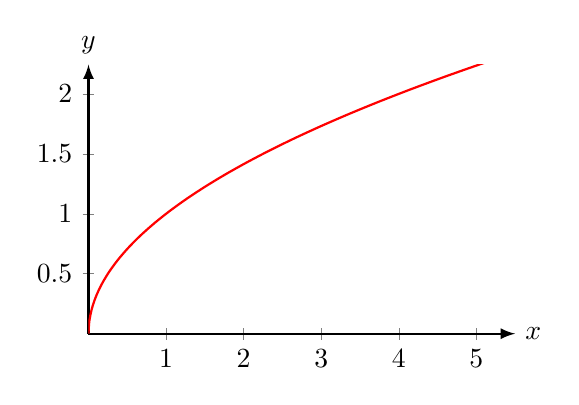
\begin{tikzpicture}
\begin{axis}[
  thick,
  width=7cm,
  height=5cm,
  domain={0}:{5},
  samples=50,
  axis y line=middle,
  axis x line=middle,
  xlabel={$x$},
  ylabel={$y$},
  xlabel style={right},
  ylabel style={above},
  xmin=0, xmax={5.5},
  ymin=0,
  ]
  \addplot[red,smooth] (x^2, x);
\end{axis}
\end{tikzpicture}
\end{document}
